%% LyX 2.4.4 created this file.  For more info, see https://www.lyx.org/.
%% Do not edit unless you really know what you are doing.
\documentclass[english,t]{beamer}
\usepackage{mathptmx}
\usepackage[T1]{fontenc}
\usepackage[latin9]{inputenc}
\usepackage{amssymb}
\usepackage{cancel}
\PassOptionsToPackage{normalem}{ulem}
\usepackage{ulem}

\makeatletter
%%%%%%%%%%%%%%%%%%%%%%%%%%%%%% Textclass specific LaTeX commands.
% this default might be overridden by plain title style
\newcommand\makebeamertitle{\frame{\maketitle}}%
% (ERT) argument for the TOC
\AtBeginDocument{%
  \let\origtableofcontents=\tableofcontents
  \def\tableofcontents{\@ifnextchar[{\origtableofcontents}{\gobbletableofcontents}}
  \def\gobbletableofcontents#1{\origtableofcontents}
}

%%%%%%%%%%%%%%%%%%%%%%%%%%%%%% User specified LaTeX commands.
\usetheme{Warsaw}
% or ...

\setbeamercovered{transparent}
% or whatever (possibly just delete it)
\setbeamercovered{invisible} %makes overlays invisible


%gets rid of navigation symbols
\setbeamertemplate{navigation symbols}{}

\usepackage{multicol}

\usepackage{tikz}
\usetikzlibrary{calc}
\usetikzlibrary{plotmarks}
\usepackage{pgfplots}
\pgfplotsset{compat=newest}

\usepackage{calc}
\usepackage[nomessages]{fp}

\usepackage{advdate}    % Advancing/saving dates
\usepackage{datetime}   % Dates formatting
\usepackage{datenumber} % Counters for dates
\usepackage[super]{nth}

\usepackage{etex}


%\usepackage{pgfpages}
%\pgfpagesuselayout{4 on 1}[a4paper, landscape, border shrink=7mm]
%\pgfpageslogicalpageoptions{1}{border code=\pgfusepath{stroke}}
%\pgfpageslogicalpageoptions{2}{border code=\pgfusepath{stroke}}
%\pgfpageslogicalpageoptions{3}{border code=\pgfusepath{stroke}}
%\pgfpageslogicalpageoptions{4}{border code=\pgfusepath{stroke}}
%%%Don't forget to add 'handout'

\makeatother

\usepackage{babel}
\begin{document}
\newcommand{\xmax}{2000}
\newcommand{\xmin}{0}
\newcommand{\xstep}{0} %must be xmin+n
\newcommand{\ymax}{500}
\newcommand{\ymin}{0}
\newcommand{\ystep}{0} %must be ymin+n

\newcounter{countEx} \setcounter{countEx}{0}
\newcounter{countProb} \setcounter{countProb}{0}
\resetcounteronoverlays{countEx} \resetcounteronoverlays{countProb}

\newcommand{\ex}[3]{
	\addtocounter{countEx}{1}
	\only<#1-#2>{\begin{exampleblock} {Example \chNum.\secNum.\arabic{countEx}.} #3	\end{exampleblock}}
}

\newcommand{\prob}[4]{
	\addtocounter{countProb}{1}
	\only<#1-#2>{\begin{exampleblock} {Problem  \chNum.\secNum.\arabic{countProb}.\,#3} #4	\end{exampleblock}}
}

\newcommand{\yline}[4]{
	(#2 - #4)/(#1 - #3)*(x - #1) + #2
}

\beamerdefaultoverlayspecification{<+->}

%%%%Chapter and Section numbers%%%%%
\newcommand{\chNum}{7}
\newcommand{\secNum}{2}
\newcommand{\secTitle}{Venn Diagrams}

\title[Section \chNum.\secNum: \secTitle]{Section \chNum.\secNum: \secTitle}

\subtitle{Finite Mathematics~~MTH 132~~Spring 2014}

\author{Dr.\,James Ashe}

%\titlegraphic{\includegraphics[height=1.5cm]{/home/jim/JamesAshe/JCSU/images/jcsu_bull}}

\institute{Johnson C. Smith University}

\date{{}}

\makebeamertitle 
\begin{frame}{Venn diagrams}

\vspace{-.5cm}

\begin{figure}
\hfill%
\begin{minipage}[t]{0.33\textwidth}%
\begin{center}

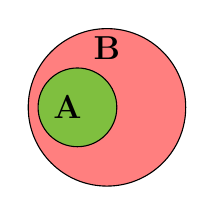
\begin{tikzpicture}     	\begin{scope}[scale=.5,shift={(3cm,-5cm)}, fill opacity=0.5,mytext/.style={text opacity=1,font=\large\bfseries}]         
		\draw[fill=red, draw = black] (0,0) circle (2);         
		\draw[fill=green, draw = black] (-0.75,0) circle (1);     
		\node[mytext] at (0,1.5) (B) {\large\textbf{B}};     		
		\node[mytext] at (-1,0) (A) {\large\textbf{A}};     	
	\end{scope}
\end{tikzpicture}
\\
\uncover<2->{$A\subseteq B$ and $A\subset B$}
\par\end{center}%
\end{minipage}\hfill%
\begin{minipage}[t]{0.33\textwidth}%
\begin{center}

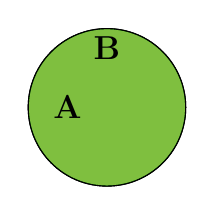
\begin{tikzpicture}     	\begin{scope}[scale=.5,shift={(3cm,-5cm)}, fill opacity=0.5,mytext/.style={text opacity=1,font=\large\bfseries}]         
		\draw[fill=red, draw = black] (0,0) circle (2);         
		\draw[fill=green, draw = black] (0.0,0) circle (2);     
		\node[mytext] at (0,1.5) (B) {\large\textbf{B}};     		
		\node[mytext] at (-1,0) (A) {\large\textbf{A}};     	
	\end{scope}
\end{tikzpicture}
\\
\uncover<3->{$A\subseteq B$}
\par\end{center}%
\end{minipage}\hfill%
\begin{minipage}[t]{0.33\textwidth}%
\begin{center}

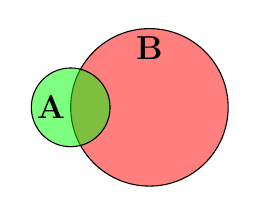
\begin{tikzpicture}     	\begin{scope}[scale=.5,shift={(3cm,-5cm)}, fill opacity=0.5,mytext/.style={text opacity=1,font=\large\bfseries}]         
		\draw[fill=red, draw = black] (0,0) circle (2);         
		\draw[fill=green, draw = black] (-2.0,0) circle (1);     
		\node[mytext] at (0,1.5) (A) {\large\textbf{B}};     		
		\node[mytext] at (-2.5,0) (B) {\large\textbf{A}};     	
	\end{scope}
\end{tikzpicture}
\\
\uncover<4->{$A\not\subset B$}
\par\end{center}%
\end{minipage}\hfill
\end{figure}

\center{\textbf{Venn Diagrams}}

\prob{5}{5}{Let $A=\{2,4,6,10\}$, $B=\{2,4,8,10\}$, $C=\{4,8,12\}$, $D=\{2,10\}$, $E=\{6\}$, and $U=\{2,4,6,8,10,12,14\}$. Insert $\subseteq$ or $\nsubseteq$ to make the statement true.}{\center $A$\underline{\hspace{.5cm}}$E$}\prob{6}{6}{Let $A=\{2,4,6,10\}$, $B=\{2,4,8,10\}$, $C=\{4,8,12\}$, $D=\{2,10\}$, $E=\{6\}$, and $U=\{2,4,6,8,10,12,14\}$. Insert $\subseteq$ or $\nsubseteq$ to make the statement true.}{\center $\emptyset$\underline{\hspace{.5cm}}$A$}\prob{7}{7}{Let $A=\{2,4,6,10\}$, $B=\{2,4,8,10\}$, $C=\{4,8,12\}$, $D=\{2,10\}$, $E=\{6\}$, and $U=\{2,4,6,8,10,12,14\}$. Insert $\subseteq$ or $\nsubseteq$ to make the statement true.}{\center $A$\underline{\hspace{.5cm}}$U$}

\prob{8}{8}{Let $A=\{2,4,6,10\}$, $B=\{2,4,8,10\}$, $C=\{4,8,12\}$, $D=\{2,10\}$, $E=\{6\}$, and $U=\{2,4,6,8,10,12,14\}$. Insert $\subseteq$ or $\nsubseteq$ to make the statement true.}{\center $A$\underline{\hspace{.5cm}}$U$}
\end{frame}

\begin{frame}{Set Operations}

\begin{columns}


\column{6cm}

\vspace{-.75cm}
\begin{block}{Union}
The \emph{union }of $A$ and $B$ is the set of all elements in $A$
\uline{or} $B$

\begin{itemize}
\item $A\cup B=\left\{ x\mid x\in A\mbox{ or }x\in B\right\} $
\end{itemize}
\end{block}

\begin{block}<4->{Intersection}
The \emph{intersection }of $A$ and $B$ is the set of all elements
in $A$ \uline{and} $B$

\begin{itemize}
\item $A\cap B=\left\{ x\mid x\in A\mbox{ and }x\in B\right\} $
\end{itemize}
\end{block}

\begin{block}<7->{Compliment}
The \emph{compliment }of $A$ is the set of everything in $U$ but
\uline{not} in $A$.

\begin{itemize}
\item $A'=\left\{ x\mid x\notin A\mbox{ and }x\in U\right\} $
\end{itemize}
\end{block}

\column{5.5cm}

%%%union%%%
\only<1-1>{%%%%A uncolored; B uncolored%%%%%
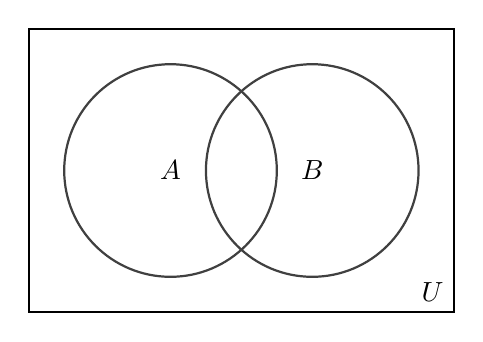
\begin{tikzpicture}[scale=.9]
	\def\circleA{(0,0) circle (1.5)} %A
	\def\circleB{(0:2) circle (1.5)} %B

	\colorlet{circle edgeA}{black!75} 
	\colorlet{circle areaA}{red!100}
	\colorlet{circle edgeB}{black!75} 
	\colorlet{circle areaB}{green!100}

	\tikzset{
		filledA/.style={fill=circle areaA, draw=circle edgeA, thick},
		filledB/.style={fill=circle areaB, draw=circle edgeB, thick},
		outlineA/.style={draw=circle edgeA, thick},
		outlineB/.style={draw=circle edgeB, thick},
	}

	\begin{scope}[fill opacity=0.5]         
			%\fill[filledB] \circleB;    
			%\fill[filledA] \circleA;
	\end{scope}

	\draw[outlineA] \circleA node {$A$}; 
	\draw[outlineB] \circleB node {$B$}; 
	%\node[anchor=south] at (current bounding box.north) {$A \cup B$}; 
	\draw[thick] (-2,-2) rectangle (4,2) node[anchor=south east] at (current bounding box.south east) {$U$}; 
\end{tikzpicture} }\only<2-2>{%%%%A colored; B uncolored%%%%%
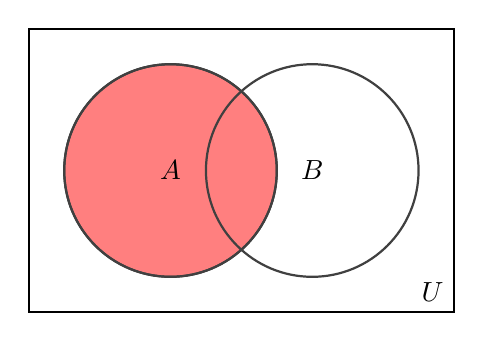
\begin{tikzpicture}[scale=.9]
	\def\circleA{(0,0) circle (1.5)} %A
	\def\circleB{(0:2) circle (1.5)} %B

	\colorlet{circle edgeA}{black!75} 
	\colorlet{circle areaA}{red!100}
	\colorlet{circle edgeB}{black!75} 
	\colorlet{circle areaB}{green!100}

	\tikzset{
		filledA/.style={fill=circle areaA, draw=circle edgeA, thick},
		filledB/.style={fill=circle areaB, draw=circle edgeB, thick},
		outlineA/.style={draw=circle edgeA, thick},
		outlineB/.style={draw=circle edgeB, thick},
	}

	\begin{scope}[fill opacity=0.5]         
			%\fill[filledB] \circleB;    
			\fill[filledA] \circleA;
	\end{scope}

	\draw[outlineA] \circleA node {$A$}; 
	\draw[outlineB] \circleB node {$B$}; 
	%\node[anchor=south] at (current bounding box.north) {$A \cup B$}; 
	\draw[thick] (-2,-2) rectangle (4,2) node[anchor=south east] at (current bounding box.south east) {$U$}; 
\end{tikzpicture} }\only<3-3>{%%%%A or B%%%%%
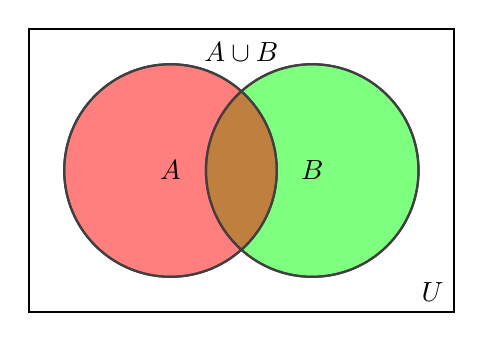
\begin{tikzpicture}[scale=.9]
	\def\circleA{(0,0) circle (1.5)} %A
	\def\circleB{(0:2) circle (1.5)} %B

	\colorlet{circle edgeA}{black!75} 
	\colorlet{circle areaA}{red!100}
	\colorlet{circle edgeB}{black!75} 
	\colorlet{circle areaB}{green!100}

	\tikzset{
		filledA/.style={fill=circle areaA, draw=circle edgeA, thick},
		filledB/.style={fill=circle areaB, draw=circle edgeB, thick},
		outlineA/.style={draw=circle edgeA, thick},
		outlineB/.style={draw=circle edgeB, thick},
	}

	\begin{scope}[fill opacity=0.5]         
			\fill[filledB] \circleB;    
			\fill[filledA] \circleA;
	\end{scope}

	\node[above=-3pt] at (current bounding box.north) {$A \cup B$}; 
	\draw[outlineA] \circleA node {$A$}; 
	\draw[outlineB] \circleB node {$B$}; 
	\draw[thick] (-2,-2) rectangle (4,2) node[anchor=south east] at (current bounding box.south east) {$U$}; 
\end{tikzpicture} }%%%intersection%%%
\only<4-4>{%%%%A colored; B uncolored%%%%%
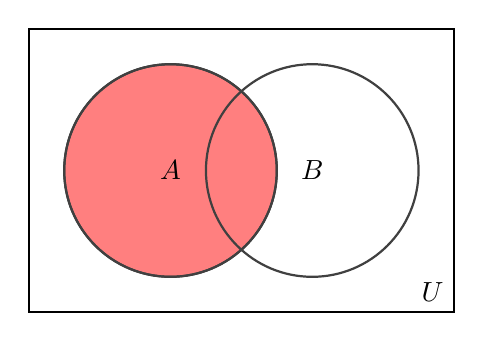
\begin{tikzpicture}[scale=.9]
	\def\circleA{(0,0) circle (1.5)} %A
	\def\circleB{(0:2) circle (1.5)} %B

	\colorlet{circle edgeA}{black!75} 
	\colorlet{circle areaA}{red!100}
	\colorlet{circle edgeB}{black!75} 
	\colorlet{circle areaB}{green!100}

	\tikzset{
		filledA/.style={fill=circle areaA, draw=circle edgeA, thick},
		filledB/.style={fill=circle areaB, draw=circle edgeB, thick},
		outlineA/.style={draw=circle edgeA, thick},
		outlineB/.style={draw=circle edgeB, thick},
	}

	\begin{scope}[fill opacity=0.5]         
			%\fill[filledB] \circleB;    
			\fill[filledA] \circleA;
	\end{scope}

	\draw[outlineA] \circleA node {$A$}; 
	\draw[outlineB] \circleB node {$B$}; 
	%\node[anchor=south] at (current bounding box.north) {$A \cup B$}; 
	\draw[thick] (-2,-2) rectangle (4,2) node[anchor=south east] at (current bounding box.south east) {$U$}; 
\end{tikzpicture} }\only<5-5>{%%%%A or B%%%%%
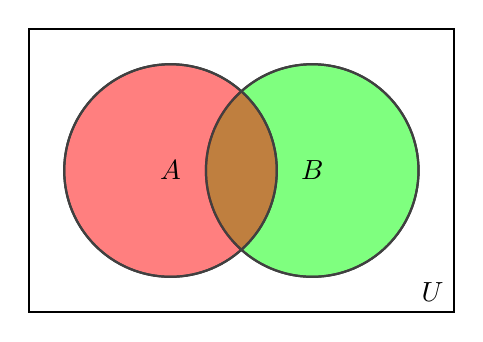
\begin{tikzpicture}[scale=.9]
	\def\circleA{(0,0) circle (1.5)} %A
	\def\circleB{(0:2) circle (1.5)} %B

	\colorlet{circle edgeA}{black!75} 
	\colorlet{circle areaA}{red!100}
	\colorlet{circle edgeB}{black!75} 
	\colorlet{circle areaB}{green!100}

	\tikzset{
		filledA/.style={fill=circle areaA, draw=circle edgeA, thick},
		filledB/.style={fill=circle areaB, draw=circle edgeB, thick},
		outlineA/.style={draw=circle edgeA, thick},
		outlineB/.style={draw=circle edgeB, thick},
	}

	\begin{scope}[fill opacity=0.5]         
			\fill[filledB] \circleB;    
			\fill[filledA] \circleA;
	\end{scope}

	\draw[outlineA] \circleA node {$A$}; 
	\draw[outlineB] \circleB node {$B$}; 
	%\node[anchor=south] at (current bounding box.north) {$A \cup B$}; 
	\draw[thick] (-2,-2) rectangle (4,2) node[anchor=south east] at (current bounding box.south east) {$U$}; 
\end{tikzpicture} }\only<6-6>{%%%%A and B%%%%%
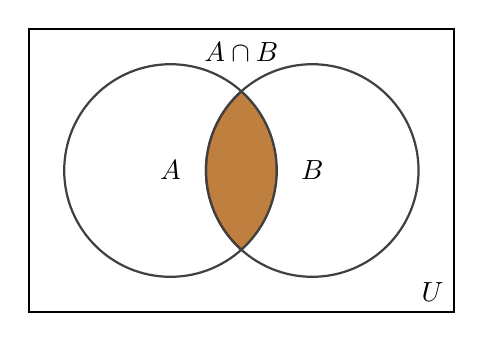
\begin{tikzpicture}[scale=.9]
	\def\circleA{(0,0) circle (1.5)} %A
	\def\circleB{(0:2) circle (1.5)} %B

	\colorlet{circle edgeA}{black!75} 
	\colorlet{circle areaA}{red!100}
	\colorlet{circle edgeB}{black!75} 
	\colorlet{circle areaB}{green!100}

	\tikzset{
		filledA/.style={fill=circle areaA, draw=circle edgeA, thick},
		filledB/.style={fill=circle areaB, draw=circle edgeB, thick},
		outlineA/.style={draw=circle edgeA, thick},
		outlineB/.style={draw=circle edgeB, thick},
	}
	
	\begin{scope}[fill opacity=0.5]    
		\clip \circleA;     
			\fill[filledB] \circleB;
		\clip \circleB;     
			\fill[filledA] \circleA;
	\end{scope}

	\draw[outlineA] \circleA node {$A$}; 
	\draw[outlineB] \circleB node {$B$}; 
	\node[above=-3pt] at (current bounding box.north) {$A \cap B$}; 
	\draw[thick] (-2,-2) rectangle (4,2) node[anchor=south east] at (current bounding box.south east) {$U$}; 
\end{tikzpicture} }%%%compliment%%%
\only<7-7>{%%%%A uncolored;%%%%%
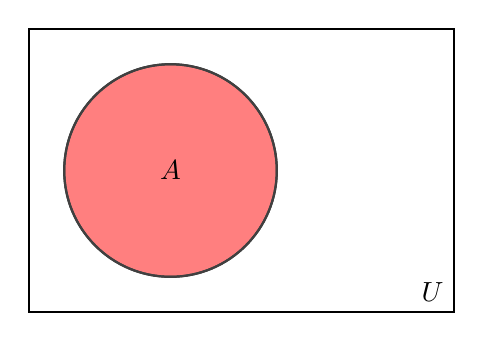
\begin{tikzpicture}[scale=.9]
	\def\circleA{(0,0) circle (1.5)} %A
	\def\circleB{(0:2) circle (1.5)} %B

	\colorlet{circle edgeA}{black!75} 
	\colorlet{circle areaA}{red!100}
	\colorlet{circle edgeB}{black!75} 
	\colorlet{circle areaB}{green!100}

	\tikzset{
		filledA/.style={fill=circle areaA, draw=circle edgeA, thick},
		filledB/.style={fill=circle areaB, draw=circle edgeB, thick},
		outlineA/.style={draw=circle edgeA, thick},
		outlineB/.style={draw=circle edgeB, thick},
	}

	\begin{scope}[fill opacity=0.5]         
			%\fill[filledB] \circleB;    
			\fill[filledA] \circleA;
	\end{scope}

	\draw[outlineA] \circleA node {$A$}; 
	%\draw[outlineB] \circleB node {$B$}; 
	%\node[anchor=south] at (current bounding box.north) {$A \cup B$}; 
	\draw[thick] (-2,-2) rectangle (4,2) node[anchor=south east] at (current bounding box.south east) {$U$}; 
\end{tikzpicture} }\only<8-8>{%%%%A compliment%%%%%
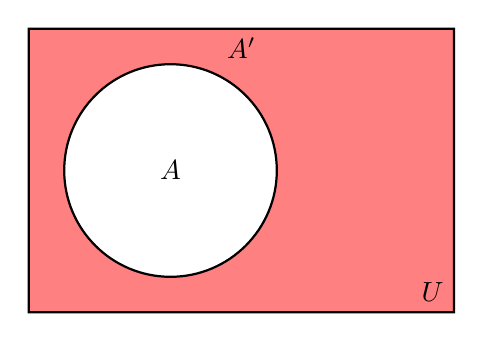
\begin{tikzpicture}[scale=.9]
	\def\circleA{(0,0) circle (1.5)} %A
	\def\circleB{(0:2) circle (1.5)} %B

	\colorlet{circle edgeA}{black!75} 
	\colorlet{circle areaA}{red!100}
	\colorlet{circle edgeB}{black!75} 
	\colorlet{circle areaB}{blue!100}

	\tikzset{
		filledA/.style={fill=circle areaA, draw=circle edgeA, thick},
		filledB/.style={fill=circle areaB, draw=circle edgeB, thick},
		outlineA/.style={draw=circle edgeA, thick},
		outlineB/.style={draw=circle edgeB, thick},
	}

	\draw[thick,fill=red!50,even odd rule] %%even odd rule draws compliment of next draw commands%%
		(-2,-2) rectangle (4,2) node[anchor=south east] at (current bounding box.south east) {$U$} 
		\circleA node {$A$};
	\node[below] at (current bounding box.north) {$A'$}; 

\end{tikzpicture} }
\end{columns}
\end{frame}

\begin{frame}{Set Operation}

\prob{1}{1}{Let $U=\{1,2,3,4,5,6,7,8,9\}$, $X=\{2,4,6,8\}$, $Y=\{2,3,4,5,6\}$, and $Z=\{1,2,3,8,9\}$. List the members of each set, using set braces.}{$X \cup Y$}

\prob{2}{2}{Let $U=\{1,2,3,4,5,6,7,8,9\}$, $X=\{2,4,6,8\}$, $Y=\{2,3,4,5,6\}$, and $Z=\{1,2,3,8,9\}$. List the members of each set, using set braces.}{$X \cap Y$}

\prob{3}{3}{Let $U=\{1,2,3,4,5,6,7,8,9\}$, $X=\{2,4,6,8\}$, $Y=\{2,3,4,5,6\}$, and $Z=\{1,2,3,8,9\}$. List the members of each set, using set braces.}{$X'$}

\prob{4}{4}{Let $U=\{1,2,3,4,5,6,7,8,9\}$, $X=\{2,4,6,8\}$, $Y=\{2,3,4,5,6\}$, and $Z=\{1,2,3,8,9\}$. List the members of each set, using set braces.}{$X' \cap Y'$}

\prob{5}{5}{Let $U=\{1,2,3,4,5,6,7,8,9\}$, $X=\{2,4,6,8\}$, $Y=\{2,3,4,5,6\}$, and $Z=\{1,2,3,8,9\}$. List the members of each set, using set braces.}{$X' \cap (Y' \cup Z)$}

\prob{6}{6}{Let $U=\{1,2,3,4,5,6,7,8,9\}$, $X=\{2,4,6,8\}$, $Y=\{2,3,4,5,6\}$, and $Z=\{1,2,3,8,9\}$. List the members of each set, using set braces.}{$(X \cap Y) \cup (X \cap Z)$}

\prob{7}{7}{Let $U=\{1,2,3,4,5,6,7,8,9\}$, $X=\{2,4,6,8\}$, $Y=\{2,3,4,5,6\}$, and $Z=\{1,2,3,8,9\}$. List the members of each set, using set braces.}{$(X \cap Y) \cap \{1,7\}$}
\end{frame}

\begin{frame}{Venn Diagram Applications}

\begin{columns}


\column{5.5cm}

\ex{1}{}{A researcher collecting data on 100 houses finds that 76 have a DVD player, 21 have a Blue Ray player, and 12 have both.}
\begin{itemize}
\item <2->How many do not have a DVD player?
\item <4->How many have neither a DVD or Blue Ray player?
\item <7->How many have a Blue Ray but not a DVD player?
\end{itemize}

\column{5.5cm}

%%%blank%%%
\only<1-2>{%%%%A uncolored; B uncolored%%%%%
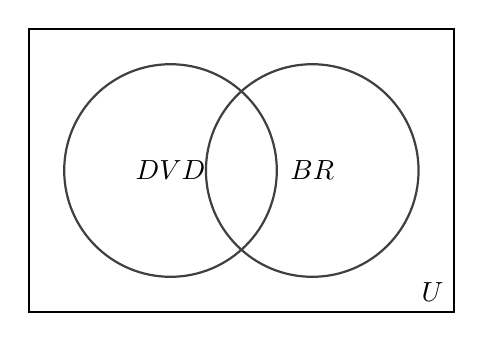
\begin{tikzpicture}[scale=.9]
	\def\circleA{(0,0) circle (1.5)} %A
	\def\circleB{(0:2) circle (1.5)} %B

	\colorlet{circle edgeA}{black!75} 
	\colorlet{circle areaA}{red!100}
	\colorlet{circle edgeB}{black!75} 
	\colorlet{circle areaB}{green!100}

	\tikzset{
		filledA/.style={fill=circle areaA, draw=circle edgeA, thick},
		filledB/.style={fill=circle areaB, draw=circle edgeB, thick},
		outlineA/.style={draw=circle edgeA, thick},
		outlineB/.style={draw=circle edgeB, thick},
	}

	\begin{scope}[fill opacity=0.5]         
			%\fill[filledB] \circleB;    
			%\fill[filledA] \circleA;
	\end{scope}

	\draw[outlineA] \circleA node {$DVD$}; 
	\draw[outlineB] \circleB node {$BR$}; 
	%\node[anchor=south] at (current bounding box.north) {$A \cup B$}; 
	\draw[thick] (-2,-2) rectangle (4,2) node[anchor=south east] at (current bounding box.south east) {$U$}; 
\end{tikzpicture} }\only<3-3>{%%%%A compliment%%%%%
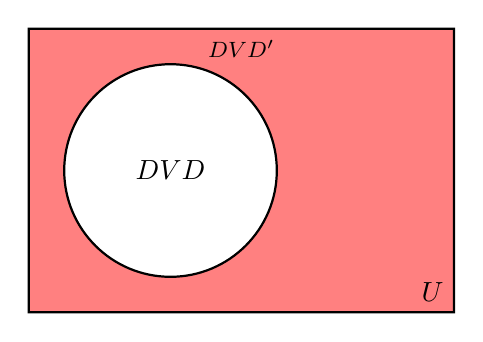
\begin{tikzpicture}[scale=.9]
	\def\circleA{(0,0) circle (1.5)} %A
	\def\circleB{(0:2) circle (1.5)} %B

	\colorlet{circle edgeA}{black!75} 
	\colorlet{circle areaA}{red!100}
	\colorlet{circle edgeB}{black!75} 
	\colorlet{circle areaB}{blue!100}

	\tikzset{
		filledA/.style={fill=circle areaA, draw=circle edgeA, thick},
		filledB/.style={fill=circle areaB, draw=circle edgeB, thick},
		outlineA/.style={draw=circle edgeA, thick},
		outlineB/.style={draw=circle edgeB, thick},
	}

	\draw[thick,fill=red!50,even odd rule] %%even odd rule draws compliment of next draw commands%%
		(-2,-2) rectangle (4,2) node[anchor=south east] at (current bounding box.south east) {$U$} 
		\circleA node {$DVD$};
	\node[below=1pt] at (current bounding box.north) {\footnotesize $DVD'$}; 

\end{tikzpicture} }%%%blank%%%
\only<4-4>{%%%%A uncolored; B uncolored%%%%%
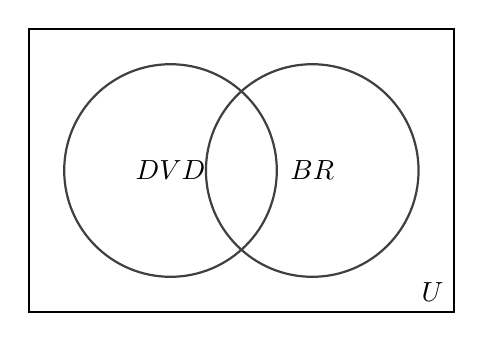
\begin{tikzpicture}[scale=.9]
	\def\circleA{(0,0) circle (1.5)} %A
	\def\circleB{(0:2) circle (1.5)} %B

	\colorlet{circle edgeA}{black!75} 
	\colorlet{circle areaA}{red!100}
	\colorlet{circle edgeB}{black!75} 
	\colorlet{circle areaB}{green!100}

	\tikzset{
		filledA/.style={fill=circle areaA, draw=circle edgeA, thick},
		filledB/.style={fill=circle areaB, draw=circle edgeB, thick},
		outlineA/.style={draw=circle edgeA, thick},
		outlineB/.style={draw=circle edgeB, thick},
	}

	\begin{scope}[fill opacity=0.5]         
			%\fill[filledB] \circleB;    
			%\fill[filledA] \circleA;
	\end{scope}

	\draw[outlineA] \circleA node {$DVD$}; 
	\draw[outlineB] \circleB node {$BR$}; 
	%\node[anchor=south] at (current bounding box.north) {$A \cup B$}; 
	\draw[thick] (-2,-2) rectangle (4,2) node[anchor=south east] at (current bounding box.south east) {$U$}; 
\end{tikzpicture} }\only<5-5>{%%%%A or B%%%%%
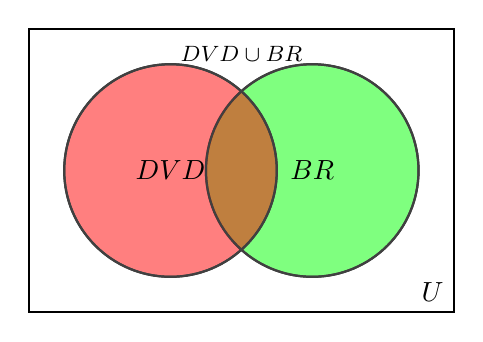
\begin{tikzpicture}[scale=.9]
	\def\circleA{(0,0) circle (1.5)} %A
	\def\circleB{(0:2) circle (1.5)} %B

	\colorlet{circle edgeA}{black!75} 
	\colorlet{circle areaA}{red!100}
	\colorlet{circle edgeB}{black!75} 
	\colorlet{circle areaB}{green!100}

	\tikzset{
		filledA/.style={fill=circle areaA, draw=circle edgeA, thick},
		filledB/.style={fill=circle areaB, draw=circle edgeB, thick},
		outlineA/.style={draw=circle edgeA, thick},
		outlineB/.style={draw=circle edgeB, thick},
	}

	\begin{scope}[fill opacity=0.5]         
			\fill[filledB] \circleB;    
			\fill[filledA] \circleA;
	\end{scope}

	\draw[outlineA] \circleA node {$DVD$}; 
	\draw[outlineB] \circleB node {$BR$}; 
	\node[above=-3pt] at (current bounding box.north) {\footnotesize $DVD \cup BR$}; 
	\draw[thick] (-2,-2) rectangle (4,2) node[anchor=south east] at (current bounding box.south east) {$U$}; 
\end{tikzpicture} }\only<6-6>{%%%%A compliment%%%%%
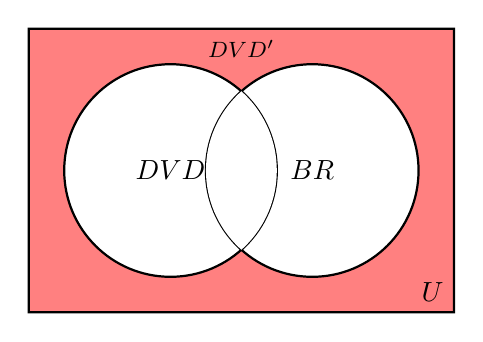
\begin{tikzpicture}[scale=.9]
	\def\circleA{(0,0) circle (1.5)} %A
	\def\circleB{(0:2) circle (1.5)} %B

	\colorlet{circle edgeA}{black!75} 
	\colorlet{circle areaA}{red!100}
	\colorlet{circle edgeB}{black!75} 
	\colorlet{circle areaB}{blue!100}

	\tikzset{
		filledA/.style={fill=circle areaA, draw=circle edgeA, thick},
		filledB/.style={fill=circle areaB, draw=circle edgeB, thick},
		outlineA/.style={draw=circle edgeA, thick},
		outlineB/.style={draw=circle edgeB, thick},
	}

		\draw[thick,fill=red!50,even odd rule] %%even odd rule draws compliment of next draw commands%%
			(-2,-2) rectangle (4,2) node[anchor=south east] at (current bounding box.south east) {$U$}
			\circleA node {$DVD$} \circleB node {$BR$};

		\scope 
			\clip (0,0) circle (1.5);%%why can't i use circleA?
			\fill[white] (0:2) circle (1.5); 
		\endscope
		
	\node[below=1pt] at (current bounding box.north) {\footnotesize $DVD'$}; 

\end{tikzpicture} }%%%blank%%%
\only<7-7>{%%%%A uncolored; B uncolored%%%%%
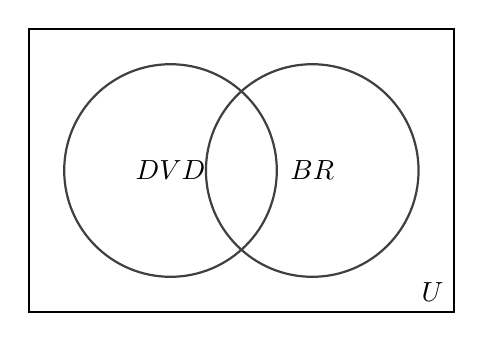
\begin{tikzpicture}[scale=.9]
	\def\circleA{(0,0) circle (1.5)} %A
	\def\circleB{(0:2) circle (1.5)} %B

	\colorlet{circle edgeA}{black!75} 
	\colorlet{circle areaA}{red!100}
	\colorlet{circle edgeB}{black!75} 
	\colorlet{circle areaB}{green!100}

	\tikzset{
		filledA/.style={fill=circle areaA, draw=circle edgeA, thick},
		filledB/.style={fill=circle areaB, draw=circle edgeB, thick},
		outlineA/.style={draw=circle edgeA, thick},
		outlineB/.style={draw=circle edgeB, thick},
	}

	\begin{scope}[fill opacity=0.5]         
			%\fill[filledB] \circleB;    
			%\fill[filledA] \circleA;
	\end{scope}

	\draw[outlineA] \circleA node {$DVD$}; 
	\draw[outlineB] \circleB node {$BR$}; 
	%\node[anchor=south] at (current bounding box.north) {$A \cup B$}; 
	\draw[thick] (-2,-2) rectangle (4,2) node[anchor=south east] at (current bounding box.south east) {$U$}; 
\end{tikzpicture} }\only<8-8>{%%%%A compliment%%%%%
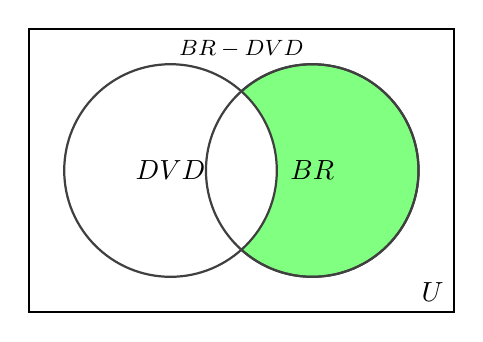
\begin{tikzpicture}[scale=.9]
	\def\circleA{(0,0) circle (1.5)} %A
	\def\circleB{(0:2) circle (1.5)} %B

	\colorlet{circle edgeA}{black!75} 
	\colorlet{circle areaA}{red!50}
	\colorlet{circle edgeB}{black!75} 
	\colorlet{circle areaB}{green!50}

	\tikzset{
		filledA/.style={fill=circle areaA, draw=circle edgeA, thick},
		filledB/.style={fill=circle areaB, draw=circle edgeB, thick},
		outlineA/.style={draw=circle edgeA, thick},
		outlineB/.style={draw=circle edgeB, thick},
	}

	\begin{scope}[shift={(6cm,0cm)}]         
		\begin{scope}[even odd rule]% B-A             
			\clip \circleA (-2,-2) rectangle (4,2);
			\fill[filledB]\circleB;         
		\end{scope}         
		\draw[outlineB] \circleB node {$BR$};         
		\draw[outlineA] \circleA node {$DVD$};
		\draw[thick] (-2,-2) rectangle (4,2) node[anchor=south east] at (current bounding box.south east) {$U$};
	\end{scope}
		
	\node[below=1pt] at (current bounding box.north) {\footnotesize $BR-DVD$}; 

\end{tikzpicture} }
\begin{block}<5->{Union Rule}
$n(A\cup B)=n(A)+n(B)-n(A\cap B)$
\end{block}
\end{columns}
\end{frame}

\begin{frame}{Venn Diagram Applications}

\begin{columns}


\column{6.5cm}

\prob{1}{}{There are 1500 students at JCSU. If 100 are math majors, 800 are female, and 75 are female math majors.}{
\begin{itemize} \item [a.] How many students are not math majors? \item [b.] How many students are both math majors and female? \item [c.] How many students are not math majors or female? \end{itemize}
}

\column{4.5cm}
\begin{block}<2->{Union Rule}
$n(A\cup B)=n(A)+n(B)-n(A\cap B)$
\end{block}
\end{columns}
\end{frame}

\begin{frame}{Venn Diagram Applications}

\begin{columns}


\column{6.5cm}

\prob{1}{}{Of the students in your class, 11 have sisters, 14 have brothers, 10 have a brother and a sister, and 5 have neither a brother or sister}{\begin{itemize} \item [a.] How many students have a brother or a sister? \item [b.] How many students are in the class? \end{itemize}}

\column{4.5cm}
\begin{block}<2->{Union Rule}
$n(A\cup B)=n(A)+n(B)-n(A\cap B)$
\end{block}
\end{columns}
\end{frame}

\begin{frame}{De Morgan's Law}

\begin{columns}


\column{5.5cm}
\begin{block}<1->{De Morgan's Law}

\begin{itemize}
\item <1->$\sim(p\wedge q)\iff\sim p\vee\sim q$
\item <7->$\sim(p\vee q)\iff\sim p\wedge\sim q$
\end{itemize}
\end{block}

\column{5.5cm}
\begin{block}<2->{De Morgan's Law}

\begin{itemize}
\item <2->$(A\cap B)'\iff A'\cup B'$
\item <8->$(A\cup B)'\iff A'\cap B'$
\end{itemize}
\end{block}
\end{columns}

\begin{columns}


\column{12cm}
\begin{center}
\only<3-3>{%%%%A and B%%%%%
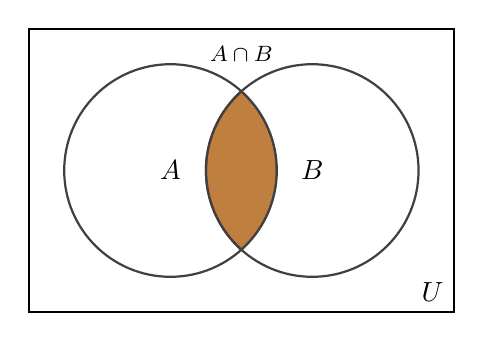
\begin{tikzpicture}[scale=.9]
	\def\circleA{(0,0) circle (1.5)} %A
	\def\circleB{(0:2) circle (1.5)} %B

	\colorlet{circle edgeA}{black!75} 
	\colorlet{circle areaA}{red!100}
	\colorlet{circle edgeB}{black!75} 
	\colorlet{circle areaB}{green!100}

	\tikzset{
		filledA/.style={fill=circle areaA, draw=circle edgeA, thick},
		filledB/.style={fill=circle areaB, draw=circle edgeB, thick},
		outlineA/.style={draw=circle edgeA, thick},
		outlineB/.style={draw=circle edgeB, thick},
	}
	
	\begin{scope}[fill opacity=0.5]    
		\clip \circleA;     
			\fill[filledB] \circleB;
		\clip \circleB;     
			\fill[filledA] \circleA;
	\end{scope}

	\draw[outlineA] \circleA node {$A$}; 
	\draw[outlineB] \circleB node {$B$}; 
	\node[above=-3pt] at (current bounding box.north) {\footnotesize  $A \cap B$}; 
	\draw[thick] (-2,-2) rectangle (4,2) node[anchor=south east] at (current bounding box.south east) {$U$}; 
\end{tikzpicture} }\only<4-4>{%%%%A and B compliment%%%%%
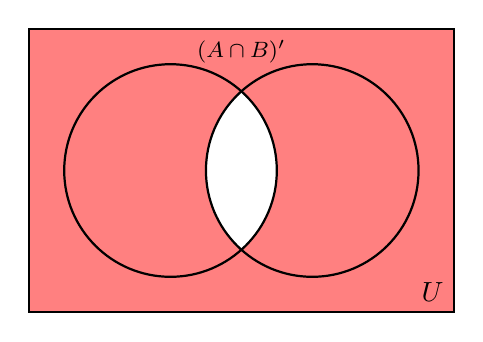
\begin{tikzpicture}[scale=.9]
	\def\circleA{(0,0) circle (1.5)} %A
	\def\circleB{(0:2) circle (1.5)} %B

	\colorlet{circle edgeA}{black!75} 
	\colorlet{circle areaA}{red!100}
	\colorlet{circle edgeB}{black!75} 
	\colorlet{circle areaB}{blue!100}

	\tikzset{
		filledA/.style={fill=circle areaA, draw=circle edgeA, thick},
		filledB/.style={fill=circle areaB, draw=circle edgeB, thick},
		outlineA/.style={draw=circle edgeA, thick},
		outlineB/.style={draw=circle edgeB, thick},
	}
		\draw[thick,fill=red!50] %%even odd rule draws compliment of next draw commands%%
			(-2,-2) rectangle (4,2) node[anchor=south east] at (current bounding box.south east) {$U$};
	
		\begin{scope}[fill opacity=1.0]    
			\clip \circleA;     
				\fill[white] \circleB;
				
			\clip \circleB;     
				\fill[white] \circleA;
				
		\end{scope}
	\draw[thick] \circleB;
	\draw[thick] \circleA;	
	\node[below=1pt] at (current bounding box.north) {\footnotesize $(A \cap B)'$}; 

\end{tikzpicture} }\only<5-6>{%%%%A compliment%%%%%
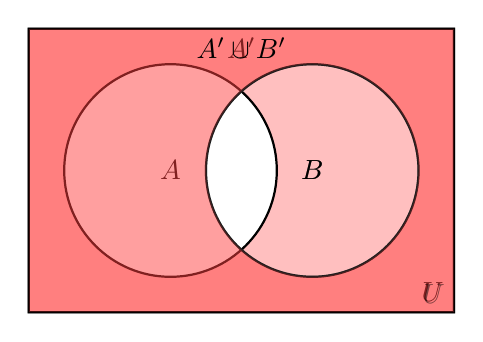
\begin{tikzpicture}[scale=.9]
	\def\circleA{(0,0) circle (1.5)} %A
	\def\circleB{(0:2) circle (1.5)} %B

	\colorlet{circle edgeA}{black!75} 
	\colorlet{circle areaA}{red!100}
	\colorlet{circle edgeB}{black!75} 
	\colorlet{circle areaB}{blue!100}

	\tikzset{
		filledA/.style={fill=circle areaA, draw=circle edgeA, thick},
		filledB/.style={fill=circle areaB, draw=circle edgeB, thick},
		outlineA/.style={draw=circle edgeA, thick},
		outlineB/.style={draw=circle edgeB, thick},
	}

	\uncover<5-6>{\draw[thick,fill=red!25,even odd rule] %%even odd rule draws compliment of next draw commands%%
		(-2,-2) rectangle (4,2) node[anchor=south east] at (current bounding box.south east) {$U$} 
		\circleA node {$A$};
		\draw[outlineB] \circleB node {$B$};
		}
	\uncover<5-5>{\node[below] at (current bounding box.north) {$A'$};}

	\uncover<6-6>{\draw[thick,fill=red!75,even odd rule,opacity=.5] %%even odd rule draws compliment of next draw commands%%
		(-2,-2) rectangle (4,2) node[anchor=south east] at (current bounding box.south east) {$U$} 
		\circleB node {$B$};}
	\uncover<6-6>{\node[below] at (current bounding box.north) {$A' \cup B'$};}

\end{tikzpicture} }\only<9-9>{%%%%A or B%%%%%
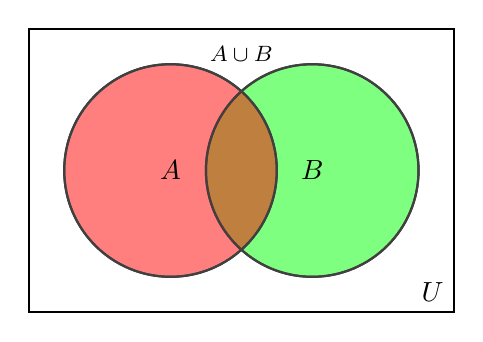
\begin{tikzpicture}[scale=.9]
	\def\circleA{(0,0) circle (1.5)} %A
	\def\circleB{(0:2) circle (1.5)} %B

	\colorlet{circle edgeA}{black!75} 
	\colorlet{circle areaA}{red!100}
	\colorlet{circle edgeB}{black!75} 
	\colorlet{circle areaB}{green!100}

	\tikzset{
		filledA/.style={fill=circle areaA, draw=circle edgeA, thick},
		filledB/.style={fill=circle areaB, draw=circle edgeB, thick},
		outlineA/.style={draw=circle edgeA, thick},
		outlineB/.style={draw=circle edgeB, thick},
	}
	
	\begin{scope}[fill opacity=0.5]    
		\fill[filledB] \circleB;
		\fill[filledA] \circleA;
	\end{scope}

	\draw[outlineA] \circleA node {$A$}; 
	\draw[outlineB] \circleB node {$B$}; 
	\node[above=-3pt] at (current bounding box.north) {\footnotesize  $A \cup B$}; 
	\draw[thick] (-2,-2) rectangle (4,2) node[anchor=south east] at (current bounding box.south east) {$U$}; 
\end{tikzpicture} }\only<10-10>{%%%%A or B compliment%%%%%
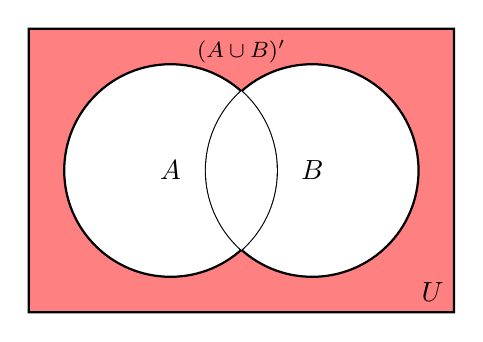
\begin{tikzpicture}[scale=.9]
	\def\circleA{(0,0) circle (1.5)} %A
	\def\circleB{(0:2) circle (1.5)} %B

	\colorlet{circle edgeA}{black!75} 
	\colorlet{circle areaA}{red!100}
	\colorlet{circle edgeB}{black!75} 
	\colorlet{circle areaB}{blue!100}

	\tikzset{
		filledA/.style={fill=circle areaA, draw=circle edgeA, thick},
		filledB/.style={fill=circle areaB, draw=circle edgeB, thick},
		outlineA/.style={draw=circle edgeA, thick},
		outlineB/.style={draw=circle edgeB, thick},
	}

		\draw[thick,fill=red!50,even odd rule] %%even odd rule draws compliment of next draw commands%%
			(-2,-2) rectangle (4,2) node[anchor=south east] at (current bounding box.south east) {$U$}
			\circleA node {$A$} \circleB node {$B$};

		\scope 
			\clip (0,0) circle (1.5);%%why can't i use circleA?
			\fill[white] (0:2) circle (1.5); 
		\endscope
		
	\node[below=1pt] at (current bounding box.north) {\footnotesize $(A \cup B)'$}; 

\end{tikzpicture} }
\par\end{center}
\end{columns}
\end{frame}

\end{document}
